\documentclass[]{article}
\usepackage{lmodern}
\usepackage{amssymb,amsmath}
\usepackage{ifxetex,ifluatex}
\usepackage{fixltx2e} % provides \textsubscript
\ifnum 0\ifxetex 1\fi\ifluatex 1\fi=0 % if pdftex
  \usepackage[T1]{fontenc}
  \usepackage[utf8]{inputenc}
\else % if luatex or xelatex
  \ifxetex
    \usepackage{mathspec}
  \else
    \usepackage{fontspec}
  \fi
  \defaultfontfeatures{Ligatures=TeX,Scale=MatchLowercase}
\fi
% use upquote if available, for straight quotes in verbatim environments
\IfFileExists{upquote.sty}{\usepackage{upquote}}{}
% use microtype if available
\IfFileExists{microtype.sty}{%
\usepackage{microtype}
\UseMicrotypeSet[protrusion]{basicmath} % disable protrusion for tt fonts
}{}
\usepackage[margin=1in]{geometry}
\usepackage{hyperref}
\hypersetup{unicode=true,
            pdftitle={®γσ, ENG LIAN HU},
            pdfauthor={®γσ, Lian Hu  ®},
            pdfborder={0 0 0},
            breaklinks=true}
\urlstyle{same}  % don't use monospace font for urls
\usepackage{longtable,booktabs}
\usepackage{graphicx,grffile}
\makeatletter
\def\maxwidth{\ifdim\Gin@nat@width>\linewidth\linewidth\else\Gin@nat@width\fi}
\def\maxheight{\ifdim\Gin@nat@height>\textheight\textheight\else\Gin@nat@height\fi}
\makeatother
% Scale images if necessary, so that they will not overflow the page
% margins by default, and it is still possible to overwrite the defaults
% using explicit options in \includegraphics[width, height, ...]{}
\setkeys{Gin}{width=\maxwidth,height=\maxheight,keepaspectratio}
\IfFileExists{parskip.sty}{%
\usepackage{parskip}
}{% else
\setlength{\parindent}{0pt}
\setlength{\parskip}{6pt plus 2pt minus 1pt}
}
\setlength{\emergencystretch}{3em}  % prevent overfull lines
\providecommand{\tightlist}{%
  \setlength{\itemsep}{0pt}\setlength{\parskip}{0pt}}
\setcounter{secnumdepth}{0}
% Redefines (sub)paragraphs to behave more like sections
\ifx\paragraph\undefined\else
\let\oldparagraph\paragraph
\renewcommand{\paragraph}[1]{\oldparagraph{#1}\mbox{}}
\fi
\ifx\subparagraph\undefined\else
\let\oldsubparagraph\subparagraph
\renewcommand{\subparagraph}[1]{\oldsubparagraph{#1}\mbox{}}
\fi

%%% Use protect on footnotes to avoid problems with footnotes in titles
\let\rmarkdownfootnote\footnote%
\def\footnote{\protect\rmarkdownfootnote}

%%% Change title format to be more compact
\usepackage{titling}

% Create subtitle command for use in maketitle
\newcommand{\subtitle}[1]{
  \posttitle{
    \begin{center}\large#1\end{center}
    }
}

\setlength{\droptitle}{-2em}

  \title{\href{https://beta.rstudioconnect.com/content/3091/ryo-eng.html}{{®γσ,
ENG LIAN HU}}}
    \pretitle{\vspace{\droptitle}\centering\huge}
  \posttitle{\par}
  \subtitle{Personal Profile}
  \author{\href{https://englianhu.github.io/}{®γσ, Lian Hu} ®}
    \preauthor{\centering\large\emph}
  \postauthor{\par}
      \predate{\centering\large\emph}
  \postdate{\par}
    \date{10/22/1984}


\begin{document}
\maketitle

{
\setcounter{tocdepth}{2}
\tableofcontents
}
\section{Curriculum Vitae}\label{curriculum-vitae}

\(®γσ\) , Eng Lian Hu

\subsection{About Me}\label{about-me}

\begin{longtable}[]{@{}lr@{}}
\toprule
\textbf{Title} & \textbf{Details}\tabularnewline
\midrule
\endhead
Date of Birth & 1984-10-22\tabularnewline
Age & 34y 0m 4d\tabularnewline
Mobile Phone Number &
\href{tel:+60172100905}{+6-017-2100905}\tabularnewline
Email Address &
\href{mailto:englianhu@gmail.com}{\nolinkurl{englianhu@gmail.com}}\tabularnewline
Nationality & Malaysian\tabularnewline
Place of Birth & Tanjong Karang, Selangor, Malaysia\tabularnewline
Religion & Buddha\tabularnewline
\bottomrule
\end{longtable}

\subsection{Education}\label{education}

\textbf{Apr-2014 to May-2016 : Professional Certificate, Specialization
Data Science}; (\href{http://www.coursera.org}{Cousera} -
\href{https://www.jhu.edu/}{Johns Hopkins University (JHU)} )

\begin{itemize}
\tightlist
\item
  \emph{01 Course title :
  \href{https://www.coursera.org/account/accomplishments/records/AjMdkzyHyA2JWRRL}{The
  Data Scientist's Toolbox}}
\item
  \emph{02 Course title :
  \href{https://www.coursera.org/account/accomplishments/certificate/VBB2XUA29B}{R
  Programming}}
\item
  \emph{03 Course title :
  \href{https://www.coursera.org/account/accomplishments/records/Q5HBLbpBekrW43Jd}{Getting
  and Cleaning Data}}
\item
  \emph{04 Course title :
  \href{https://www.coursera.org/account/accomplishments/records/4Gz8BmPsnuknW93A}{Exploratory
  Data Analysis}}
\item
  \emph{05 Course title :
  \href{https://www.coursera.org/account/accomplishments/records/xpNfvxWs8uMMYrjs}{Reproducible
  Research}}
\item
  \emph{06 Course title :
  \href{https://www.coursera.org/account/accomplishments/records/jXzs4bAFXZfJ3Dne}{Statistical
  Inference}}
\item
  \emph{07 Course title :
  \href{https://www.coursera.org/account/accomplishments/records/Su7PgrMXVGYrU4cM}{Regression
  Models}}
\item
  \emph{08 Course title :
  \href{https://www.coursera.org/account/accomplishments/records/j6DpQhLYeRj54dvS}{Practical
  Machine Learning}}
\item
  \emph{09 Course title :
  \href{https://www.coursera.org/account/accomplishments/records/ERvuyAZm6CG45EUS}{Developing
  Data Products}}
\item
  \emph{10 Course title :
  \href{https://www.coursera.org/account/accomplishments/specialization/RRYWVWNAP5EB}{Data
  Science Capstone}}
\item
  \href{https://www.coursera.org/account/accomplishments/specialization/RRYWVWNAP5EB}{\textbf{Data
  Science Specialization}}
\end{itemize}

\textbf{Jun-2015 to Aug-2015 : Professional Certificate, Specialization
Data Science}; (\href{http://www.coursera.org}{Cousera} -
\href{https://www.umich.edu/}{University of Michigan (UM)})

\begin{itemize}
\tightlist
\item
  \emph{Course title :
  \href{https://www.coursera.org/account/accomplishments/records/GA4cGW59ETHAevCa}{Programming
  for Everybody (Python)}}
\end{itemize}

\textbf{Mar-2002 to Dec-2003 : Professional Certificate, Japanese
Language Profeciency Test}; (\href{http://www.jlpt.jp/index.html}{JLPT}
- \href{http://www.jfkl.org.my/}{Japan Foundation Kuala Lumpur} and
\href{http://www.jees.or.jp/index.htm}{Japan Educational Exchanges and
Services} )

\begin{itemize}
\tightlist
\item
  \emph{Course title :
  \href{https://raw.githubusercontent.com/scibrokes/owner/master/documents/JLPT\%20Certificate.jpg}{Japanese
  Language Profeciency Test - Level III}}
\end{itemize}

\subsection{Experience}\label{experience}

\textbf{Nov-2017 to May-2018 : Customer Service Executive};(employed by
\href{http://www.aristocrat-rh.com/}{Aristocrat \& Residence} ) (2nd job
employed by \href{https://www.7liveasia88.com}{7LiveAsia} )

\begin{itemize}
\tightlist
\item
  \emph{Job Task : Work in Cambodia, a customer service executive but
  some times need to handle anti-fraud.}
\end{itemize}

\textbf{May-2016 to Dec-2016 : Customer Service Executive};(employed by
\href{http://www.manpower.com.my/}{Manpower Human Resource Sdn Bhd} and
deployed by \href{https://www.mindpearl.com/}{Mindpearl} )

\begin{itemize}
\tightlist
\item
  \emph{Job Task : A customer service executive in Mindpearl but handle
  \href{https://www.malaysiaairlines.com/my/en.html}{Malaysia Airlines}
  customers, need to handle Malaysia Airlines customers. General
  enquiry, new booking, booking amendment.}
\end{itemize}

\textbf{Oct-2015 to Jan-2016 : Online Gaming, Sportsbook Trader};
(employed by Global Solution Sdn Bhd)

\begin{itemize}
\tightlist
\item
  \emph{Job Task : Follow (Back) sportsbook punters' bets, hedging and
  oppose (Lay) pathological gamblers, doing deposit transactions for
  China mainland customers.}
\end{itemize}

\textbf{May-2015 to Sep-2015 : Online Gaming, Customer Service};
(employed by OneMedia Sdn Bhd)

\begin{itemize}
\tightlist
\item
  \emph{Job Task : Handling inbound and outbound calls, livechat,
  feedback, all deposit and withdrawal transactions.}
\end{itemize}

\textbf{Feb-2015 to Apr-2015 : Online Retails, Fraud Prevention};
(employed by \href{http://www.idealseed.com/}{IdealSeed Sdn Bhd} and
deployed by \href{http://www.apple.com}{Apple Inc.} )

\begin{itemize}
\tightlist
\item
  \emph{Job Task : Working in \href{https://www.xerox.com/}{Xerox}
  office. Handling inbound and outbound calls, check and approve/reject
  customers' ordered transactions.}
\end{itemize}

\textbf{Mar-2014 to Apr-2014 : Customer Service Executive}; (employed by
\href{https://www.fujixerox.com}{FujiXerox} )

\begin{itemize}
\tightlist
\item
  \emph{Job Task : Handling inbound calls from Taiwanese customers'
  orders and printer maintenance.}
\end{itemize}

\textbf{Nov-2013 to Mar-2014 : Online Gaming Trading, Team
Leader/Trader}; ( employed by
\href{http://www.gb-links.com/}{SBSolutionCorp Ltd} )

\begin{itemize}
\tightlist
\item
  \emph{Job Task : Handling few members to update scores and bets
  settlement.}
\end{itemize}

\textbf{Nov-2012 to May-2013 : TV Broadcasting Channel, Video Editor};
(employed by \href{http://www.udrive-media.com/}{U-Drive Media Sdn Bhd}
)

\begin{itemize}
\tightlist
\item
  \emph{Job Task : Watching and filtering video streaming from abroad
  prior to play in our country. \href{https://tm.com.my/\#/explore}{TM
  Bhd} Telekom Malaysia project}
\end{itemize}

\textbf{Mar-2008 to Jul-2012 : Outsourcing Business, Customer Service};
(employed by \href{http://www.scicom-intl.com/}{Scicom (MSC) Bhd} )

\begin{itemize}
\tightlist
\item
  \emph{Job Task : Handling inbound and outbound calls, livechat,
  feedback, all deposit, withdrawal and also phone bets' transactions.
  Sometimes need to do translation and also analysis job tasks.
  \href{http://www.ladbrokesplc.com/}{Ladbrokes PLC}'s project}
\item
  Awarded
  \href{https://raw.githubusercontent.com/scibrokes/owner/master/documents/Scicom\%20CS\%20Workshop.jpg}{Customer
  Service Workshop}
\item
  Awarded
  \href{https://raw.githubusercontent.com/scibrokes/owner/master/documents/Scicom\%20Appreciation\%20Certificate.jpg}{(Ladbrokes)
  Appreciation Certificate.jpg}
\end{itemize}

\textbf{Jul-2006 to Jun-2007 : Online Gambling, Trainer/Trader};
(employed by
\href{http://www.callcenterbeat.com/caspo-philippines/}{Caspo Inc.} )

\begin{itemize}
\tightlist
\item
  \emph{Job Task : Provides training to newbies on sportsbook trading
  and live scout. Need to backup for trading as well. Sometimes need to
  do translation and also analysis job tasks.}
\end{itemize}

\textbf{Nov-2005 to Jul-2006 : Online Gambling, Team Leader/Senior
Trader}; (employed by \href{http://www.telebizness.com/}{Telebiz Sdn
Bhd} )

\begin{itemize}
\tightlist
\item
  \emph{Job Task : Provides training to newbies on sportsbook trading
  purchasing stocks, need to update scores for bets financial
  settlement. Handle live-matches on corners. Sometimes need to do
  translation and also analysis job tasks.}
\end{itemize}

\subsection{Technical Experience}\label{technical-experience}

\href{https://github.com/scibrokes/analyse-the-finance-and-stocks-price-of-bookmakers}{\textbf{Analysing
Financial Report of Bookmakers}}

\begin{itemize}
\tightlist
\item
  \emph{Analyse the financial report and stock price of gambling public
  listed company.}
\item
  \emph{Analyse the profit and loss of Singbet and Singbet2.}
\item
  \emph{Kindly click
  \href{https://github.com/scibrokes/analyse-the-finance-and-stocks-price-of-bookmakers}{here}
  for more information.}
\end{itemize}

\href{https://github.com/englianhu/binary.com-interview-question}{\textbf{binary.com
: Job Application - Quantitative Analyst}}

\begin{itemize}
\tightlist
\item
  \emph{Backtest on financial betting products modelling and also
  betting strategy.}
\item
  \emph{Backtest on application of Arima, Exponential Smoothing model,
  and various Garch models for prediction and Kelly model for
  investment.}
\item
  \emph{Imputation of missing value dataset and backtest on high
  frequency trading.}
\item
  \emph{Kindly click
  \href{https://github.com/englianhu/binary.com-interview-question}{here}
  for more information.}
\end{itemize}

\href{https://github.com/Scibrokes/Betting-Strategy-and-Model-Validation}{\textbf{Betting
Strategy and Model Validation}}

\begin{itemize}
\tightlist
\item
  \emph{Using Selenium to gather soccer matches data via webdriver
  Phantomjs.}
\item
  \emph{Natural language analysis on the scrapped livescore data to
  match the team names from firm A for automation soccer team name
  matching.}
\item
  \emph{Application of different leverage of Kelly criterion for
  staking.}
\item
  \emph{Kindly click
  \href{https://github.com/Scibrokes/Betting-Strategy-and-Model-Validation}{here}
  for more information.}
\end{itemize}

\href{https://github.com/Scibrokes/setup-rstudio-server}{\textbf{Introducing
®Studio Server for Data Scientists}}

\begin{itemize}
\tightlist
\item
  \emph{An tutorial for setup RStudio server and shiny server on Linux
  CentOS 7.}
\item
  \emph{Kindly click
  \href{https://github.com/Scibrokes/setup-rstudio-server}{here} for
  more information.}
\end{itemize}

\href{https://github.com/Scibrokes/kelly-criterion}{\textbf{Application
of Kelly Criterion model in Sportsbook Investment}}

\begin{itemize}
\tightlist
\item
  \emph{Apply dynamic weighted diagonal inflated bivariate poisson model
  to the scrapped data from} \textbf{WebDriver Dynamic Webpage
  Scrapping} \emph{to build an prediction model.}
\item
  \emph{Application of Kelly criterion model to betting on 10
  sportsbookmakers in soccer season 2011/12 to 2012/13.}
\item
  \emph{Kindly click
  \href{https://github.com/Scibrokes/kelly-criterion}{here} for more
  information.}
\end{itemize}

\href{https://github.com/Scibrokes/Dixon-Coles1996}{\textbf{Dixon-Coles1996}}

\begin{itemize}
\tightlist
\item
  \emph{Dixon \& Coles 1996 soccer scores modelling.}
\item
  \emph{Kindly click
  \href{https://github.com/Scibrokes/Dixon-Coles1996}{here} for more
  information.}
\end{itemize}

\href{https://github.com/Scibrokes/WebDriver-DynamicWebpage-Scrapping}{\textbf{WebDriver
Dynamic Webpage Scrapping}}

\begin{itemize}
\tightlist
\item
  \emph{Application of RSelenium and Python to scrape the odds price of
  sportbookmakers and also livescore data from}
  \href{http://odds.7m.hk/en/}{\emph{7M}} \emph{and}
  \href{http://info.nowgoal.com/en/}{\emph{NowGoal}} \emph{website as
  well as filter the odds price data.}
\item
  \emph{Kindly click
  \href{https://github.com/Scibrokes/WebDriver-DynamicWebpage-Scrapping}{here}
  for more information.}
\end{itemize}

\href{https://github.com/Scibrokes/Soccer-League-Web-Scraping}{\textbf{Soccer
League Web Scraping}}

\begin{itemize}
\tightlist
\item
  \emph{Static webpage soccer scores scraping.}
\item
  \emph{Kindly click
  \href{https://github.com/Scibrokes/Soccer-League-Web-Scraping}{here}
  for more information.}
\end{itemize}

\href{https://github.com/scibrokes/odds-modelling-and-testing-inefficiency-of-sports-bookmakers}{\textbf{Odds
Modelling and Testing Inefficiency of Sports-Bookmakers}}

\begin{itemize}
\tightlist
\item
  \emph{Collect the livescore and also 1x2, Asian Handicap, Over Under
  odds price data of 29 sportsbookmakers manually from}
  \href{http://www.500wan.com}{\emph{500WAN}},
  \href{http://www.bet007.com}{\emph{BET007}} \emph{and}
  \href{http://info.nowgoal.com/en/}{\emph{NowGoal}} \emph{website and
  filter the odds price data from 2006 to 2011.}
\item
  \emph{Apply dynamical weighted diagonal inflated bivariate Poisson
  model in R to test the return of the investment.}
\item
  \emph{Kindly click
  \href{https://github.com/scibrokes/odds-modelling-and-testing-inefficiency-of-sports-bookmakers}{here}
  for more information.}
\end{itemize}

\href{https://www.dropbox.com/sh/h3e6gv59onz311j/AAAFcfFOfon-kEhveTzvHGHza?dl=0}{\textbf{Apply
Poisson regression on sports odds modelling}}

\begin{itemize}
\tightlist
\item
  \emph{Application of Poison model onto soccer sports odds modelling.}
\item
  \emph{Kindly click on
  \href{https://github.com/scibrokes/owner/blob/master/data/Calculator.xls}{Calculator.xls}
  and
  \href{https://github.com/scibrokes/owner/blob/master/data/Statistics\%20(ver3).xls}{Statistics
  (ver3).xls} for the research.}
\end{itemize}

\subsection{Skill}\label{skill}

Skill and Expertise

Skill and Expertise Rating Level (from newbie 1 to expert 10)

\hypertarget{htmlwidget-9b4f2ba90894d7bf44fd}{}

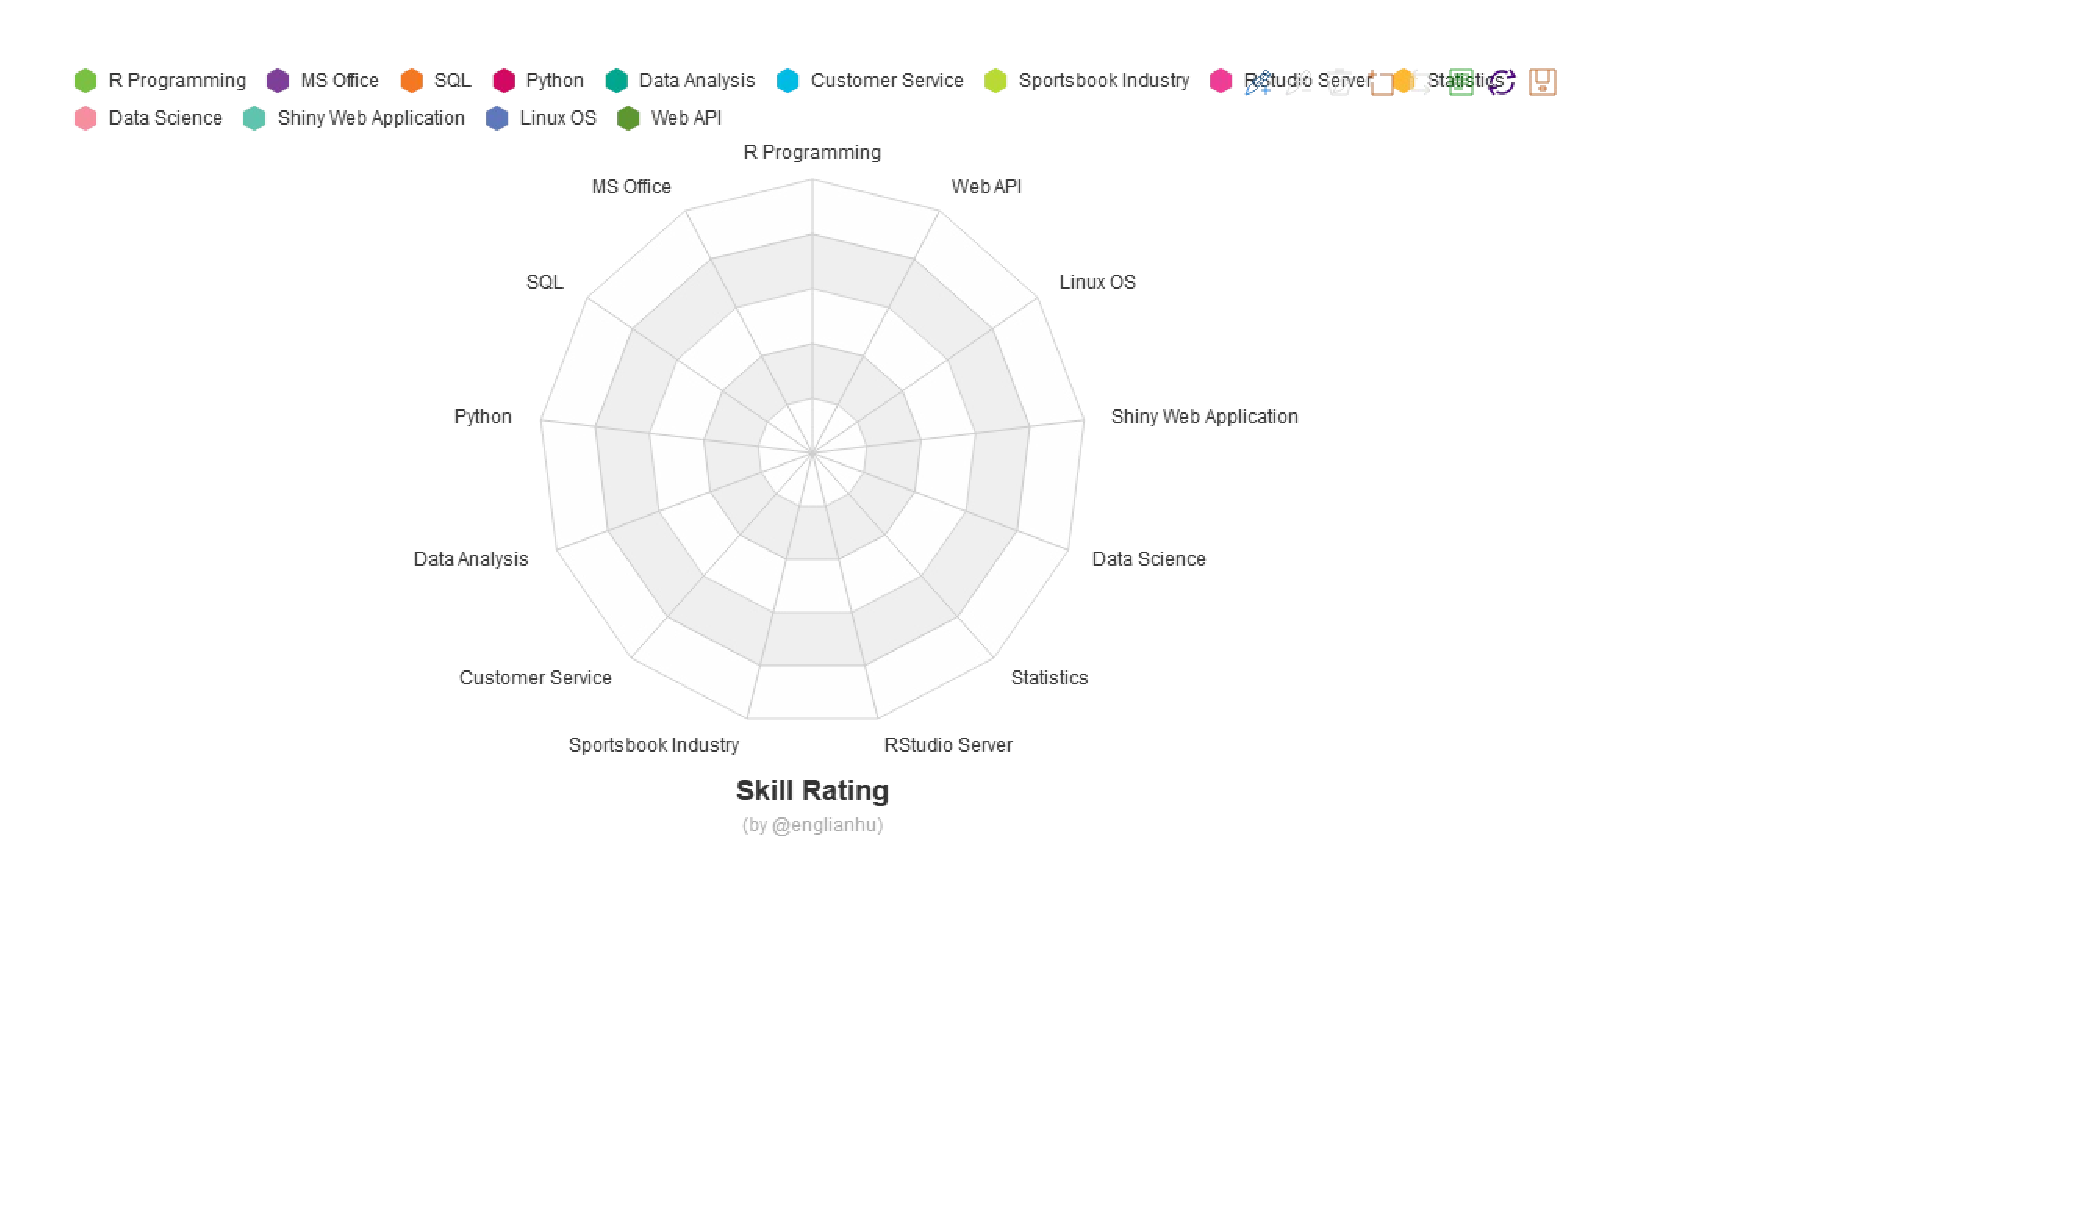
\includegraphics{ryo-eng_files/figure-latex/skill2-1.pdf}
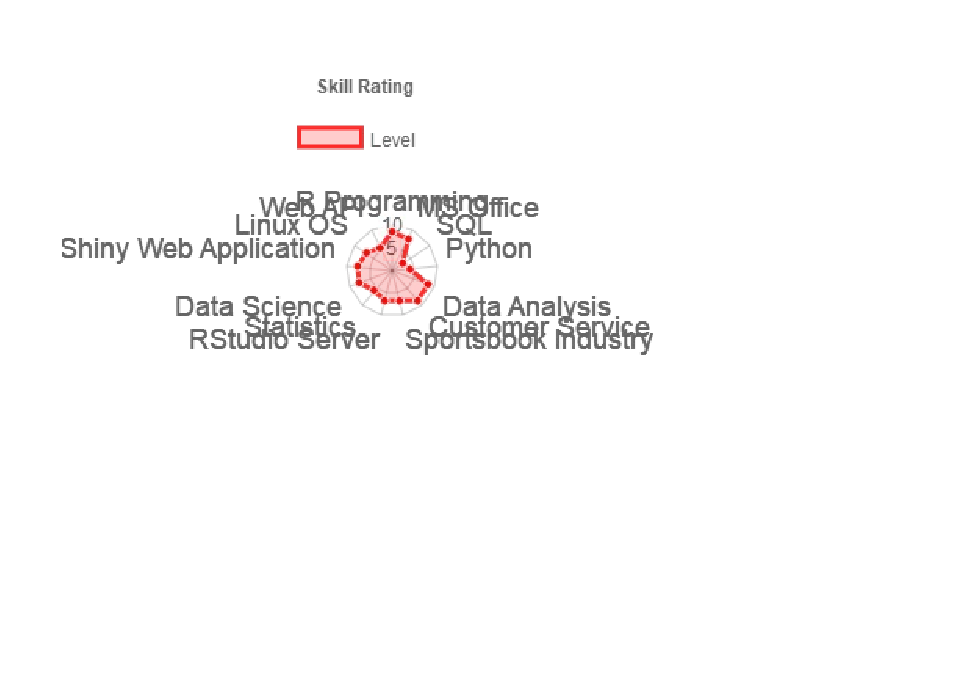
\includegraphics{ryo-eng_files/figure-latex/skill2-2.pdf}

\subsection{Other / Miscellaneous}\label{other-miscellaneous}

I am currently learn to setup own sportsbook hedge fund company
\href{https://github.com/scibrokes}{Scibrokes®}\footnote{The website not
  yet setup but now keep up learning.} which will be the first
professional sportsbook hedge fund in Asia I though. You are welcome to
own yours by refer to my
\href{https://github.com/Scibrokes/setup-rstudio-server}{安装
®StudioとShiny服务器} . You are welcome to contact me at
\href{mailto:englianhu@gmail.com}{\nolinkurl{englianhu@gmail.com}}.

\subsection{Social Network}\label{social-network}

\section{Appendices}\label{appendices}

\subsection{Documenting File Creation}\label{documenting-file-creation}

It's useful to record some information about how your file was created.

\begin{itemize}
\tightlist
\item
  File creation date: 2015-10-12
\item
  R version 3.5.1 (2018-07-02)
\item
  R version (short form): 3.5.1
\item
  \href{https://github.com/rstudio/rmarkdown}{\textbf{rmarkdown}}
  package version: 1.10
\item
  File version: 1.0.1
\item
  File latest updated date: 2018-10-26
\item
  Author Profile:
  \href{https://beta.rstudioconnect.com/content/3091/ryo-eng.html}{®γσ,
  Eng Lian Hu}
\item
  GitHub: \href{https://github.com/scibrokes/owner}{Source Code}
\item
  Additional session information
\end{itemize}

Additional session information:

Category

session\_info

Category

Sys.info

version

R version 3.5.1 (2018-07-02)

sysname

Windows

os

Windows 10 x64

release

10 x64

system

x86\_64, mingw32

version

build 17134

ui

RTerm

nodename

RSTUDIO-SCIBROK

language

en

machine

x86-64

collate

Japanese\_Japan.932

login

scibr

ctype

Japanese\_Japan.932

user

scibr

tz

Asia/Tokyo

effective\_user

scibr

date

2018-10-26

Current time

2018-10-26 15:18:54 JST

\subsection{References}\label{references}

\begin{itemize}
\tightlist
\item
  You are feel free to create your own CV by R Markdown V2 by refer to
  \href{http://rmarkdown.rstudio.com/developer_document_templates.html?version=0.99.484\&mode=server}{Document
  Templates}
\item
  \href{http://yixuan.cos.name/prettydoc/}{prettydoc}
\item
  \href{http://rmarkdown.rstudio.com/authoring_pandoc_markdown.html}{Pandoc
  Markdown}
\item
  You can plot a
  \href{http://stackoverflow.com/questions/20695311/chronological-timeline-with-points-in-time-and-format-date}{timeline}
  graph or load the \href{http://jason.bryer.org/timeline/}{timeline}
  package.
\item
  Here I apply
  \href{https://cran.r-project.org/web/packages/googleVis/vignettes/Using_googleVis_with_knitr.html}{googleVis}
  package to plot the animated graph. You are feel free to browse over
  the
  \href{https://cran.r-project.org/web/packages/googleVis/vignettes/googleVis.pdf}{vignettes}
  for more examples.
\item
  You can also modify the layout of website by referring
  \href{http://rstudio-pubs-static.s3.amazonaws.com/27777_55697c3a476640caa0ad2099fe914ae5.html\#/}{Top
  Five CSS Customizations for R Presentations}.
\item
  There are a lot of diversified symbols I get from
  \href{http://www.rapidtables.com/math/symbols/greek_alphabet.htm}{Greek
  Alphabet Symbols}
\end{itemize}

\begin{center}\rule{0.5\linewidth}{\linethickness}\end{center}

{\textbf{Powered by - Copyright® Intellectual Property Rights of
\href{http://www.scibrokes.com}{®}個人の経営企業}}


\end{document}
